\documentclass[12pt]{article}
\usepackage[utf8]{inputenc}
\usepackage{fancyhdr}
\usepackage[includehead, margin=2cm]{geometry}
\usepackage{listings}
\usepackage{titling}
\usepackage{parskip}
\usepackage{fancyvrb}
\usepackage{tabularx}
\usepackage{float}
\usepackage{hyperref}
\usepackage{graphicx}


\usepackage{xcolor}
\lstset{basicstyle=\ttfamily,
  showstringspaces=false,
  commentstyle=\color{red},
  keywordstyle=\color{blue}
}
\newcommand{\codeIn}[1]{{\small\tt{#1}}}
\hypersetup{
    colorlinks=true,
    urlcolor=blue
}

\pagestyle{fancy}

\newenvironment{centeredcode}
{
\ttfamily
\begin{center}
\begin{tabular}{l}
}
{
\end{tabular}
\end{center}
}

\newcommand{\classTitle}{CS 6340: Software Analysis and Test, Fall 2023}
\newcommand{\projectTitle}{SVF Project}
\newcommand{\implementationFile}{\codeIn{project.cpp} }
\newcommand{\src}{\codeIn{src}}
\newcommand{\sink}{\codeIn{sink}}


\title{
\classTitle
\Large
\\
\projectTitle
}
\preauthor{}
\postauthor{}
\author{}
\date{}

\begin{document}
\lhead{\classTitle}
\rhead{\projectTitle}
\maketitle
\thispagestyle{fancy}


\section{Project Description}

In this project, you will get familiar with the \href{https://svf-tools.github.io/SVF}{SVF} framework, and build a reachability analysis tool working on \href{https://llvm.org/docs/LangRef.html#instruction-reference}{LLVM IR}. SVF is a static tool that enables scalable and precise interprocedural dependence analysis on LLVM IRs. Your submitted analysis tool should read LLVM IR files and decide (statically) whether the function call \src () reaches the function call \sink ().



\subsection{Task Description}
An interprocedural control-flow graph (ICFG)  describes the control flow of a target program. The ICFG represents the control instructions from the program entry node to the program exit node and provides multiple control flows among the whole program. Analysis of an ICFG can be used to detect path reachability between two nodes. 

\begin{figure*}[htpb]
    \centering
    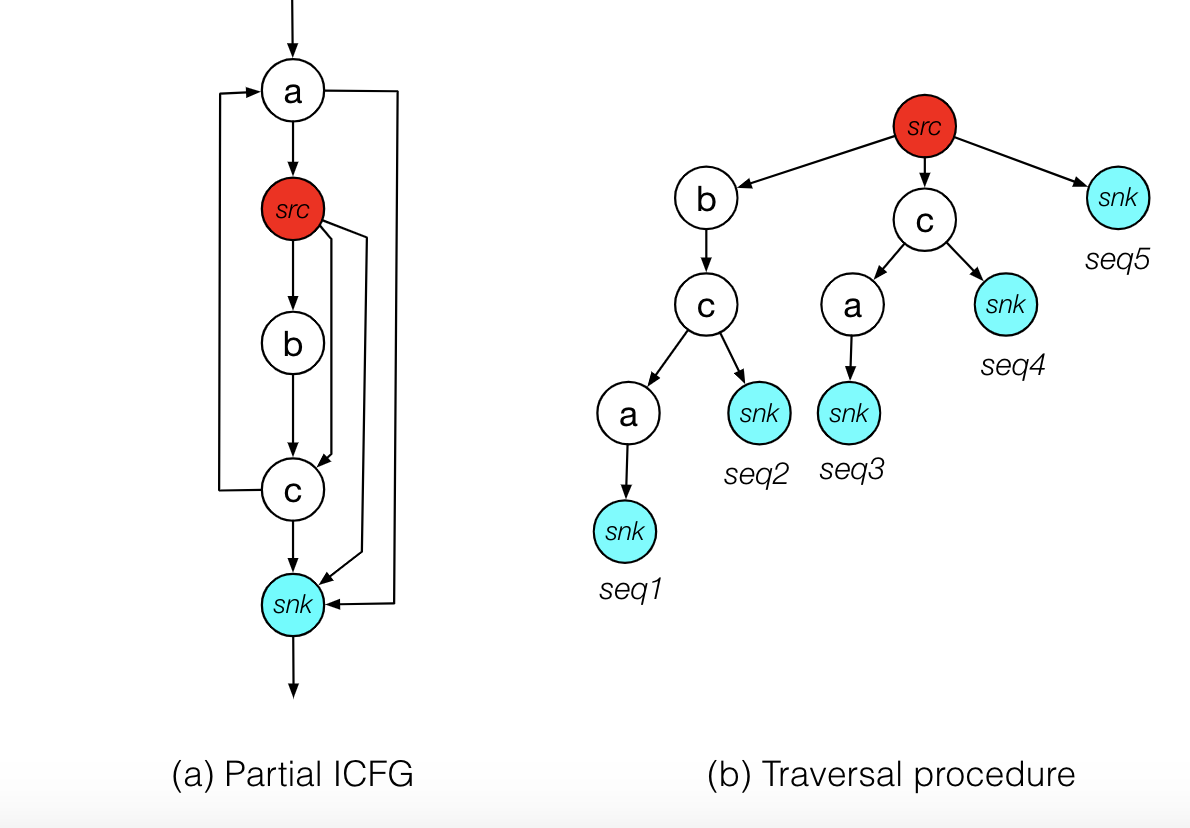
\includegraphics[scale=0.6]{icfgCase1.png}
    \caption{Example}
    \label{case1}
\end{figure*}


Your program should perform the previously mentioned reachability analysis.
Some caveats:
\begin{enumerate}
    \item The analysis should be \textbf{Path-Insensitive \& Context-Sensitive}. No data flow analysis is necessary. As such, paths that are infeasible can appear in your output:
\begin{figure*}[htpb]
    \centering
    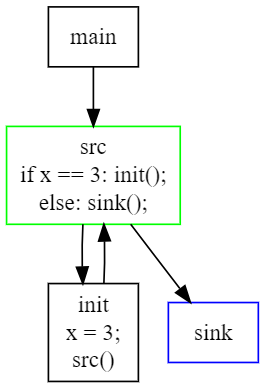
\includegraphics[scale=0.6]{interprocedural.png}
    \caption{Interprocedural Case}
    \label{case1}
\end{figure*}

    \begin{enumerate}
        \item \codeIn{$src-->sink$} (infeasible)
        \item \codeIn{$src-->init-->src-->sink$}
        \item \codeIn{$Cycle[src-->init-->src]-->sink$} (infeasible)
        \item \codeIn{$src-->Cycle[init-->src]-->sink$} (infeasible)
    \end{enumerate}

    \item You do not need to consider recursive function call cycles in this project.
    
\end{enumerate}
The ICFG can be generated by the SVF framework; SVF also provides the functionality to identify instructions represented by the nodes in the ICFG.

One goal in this project is also to learn how to utilize
a real-world static analysis framework to implement analysis
tools. Please start early to get familiar with the SVF framework in this project!
Reference for the SVF framework is available at \url{https://github.com/SVF-tools/SVF/wiki}.

\subsection{Project Setup}\label{sec:setup}

\subsubsection{Docker}
To avoid any configuration issues, we will use \href{https://www.docker.com/}{Docker} in this project. We provide a guide to use Docker in your project, and our grading environment will be the same as described in the guide. Here are the instructions to set up, build and test your project.

First you need to install Docker on your local machine. Here is the link to help to get started with Docker: \url{https://www.docker.com/get-started}.

Once you have Docker installed on your machine, you can pull the provided Docker image from Docker Hub and then work on it. Here is a guide of the entire process. If you want to know more about Docker please consult the official documentation.

\begin{enumerate}
    \item First you can pull the image from Docker Hub.\\\\
    \codeIn{docker pull mdavis438/svfproject:latest}\\
    \item Then you can start a Docker container from the provided Docker image using the following command.\\\\
    \codeIn{docker run -it --name svfproject cs4240/project3:latest /bin/bash}\\\\
    If you want to come back later you can exit the bash session and start the stopped container again using the following command.\\\\
    \codeIn{docker start -ai svfproject}\\\\
\end{enumerate}

\subsubsection{VSCode (optional)}

This section provides a guide for if you want to use VScode dev container connections.

\begin{enumerate}
    \item Install VSCode Editor: \url{https://code.visualstudio.com/download}
    
    \item Install Remote Development Extension in VSCode
    \begin{figure*}[htpb]
        \centering
        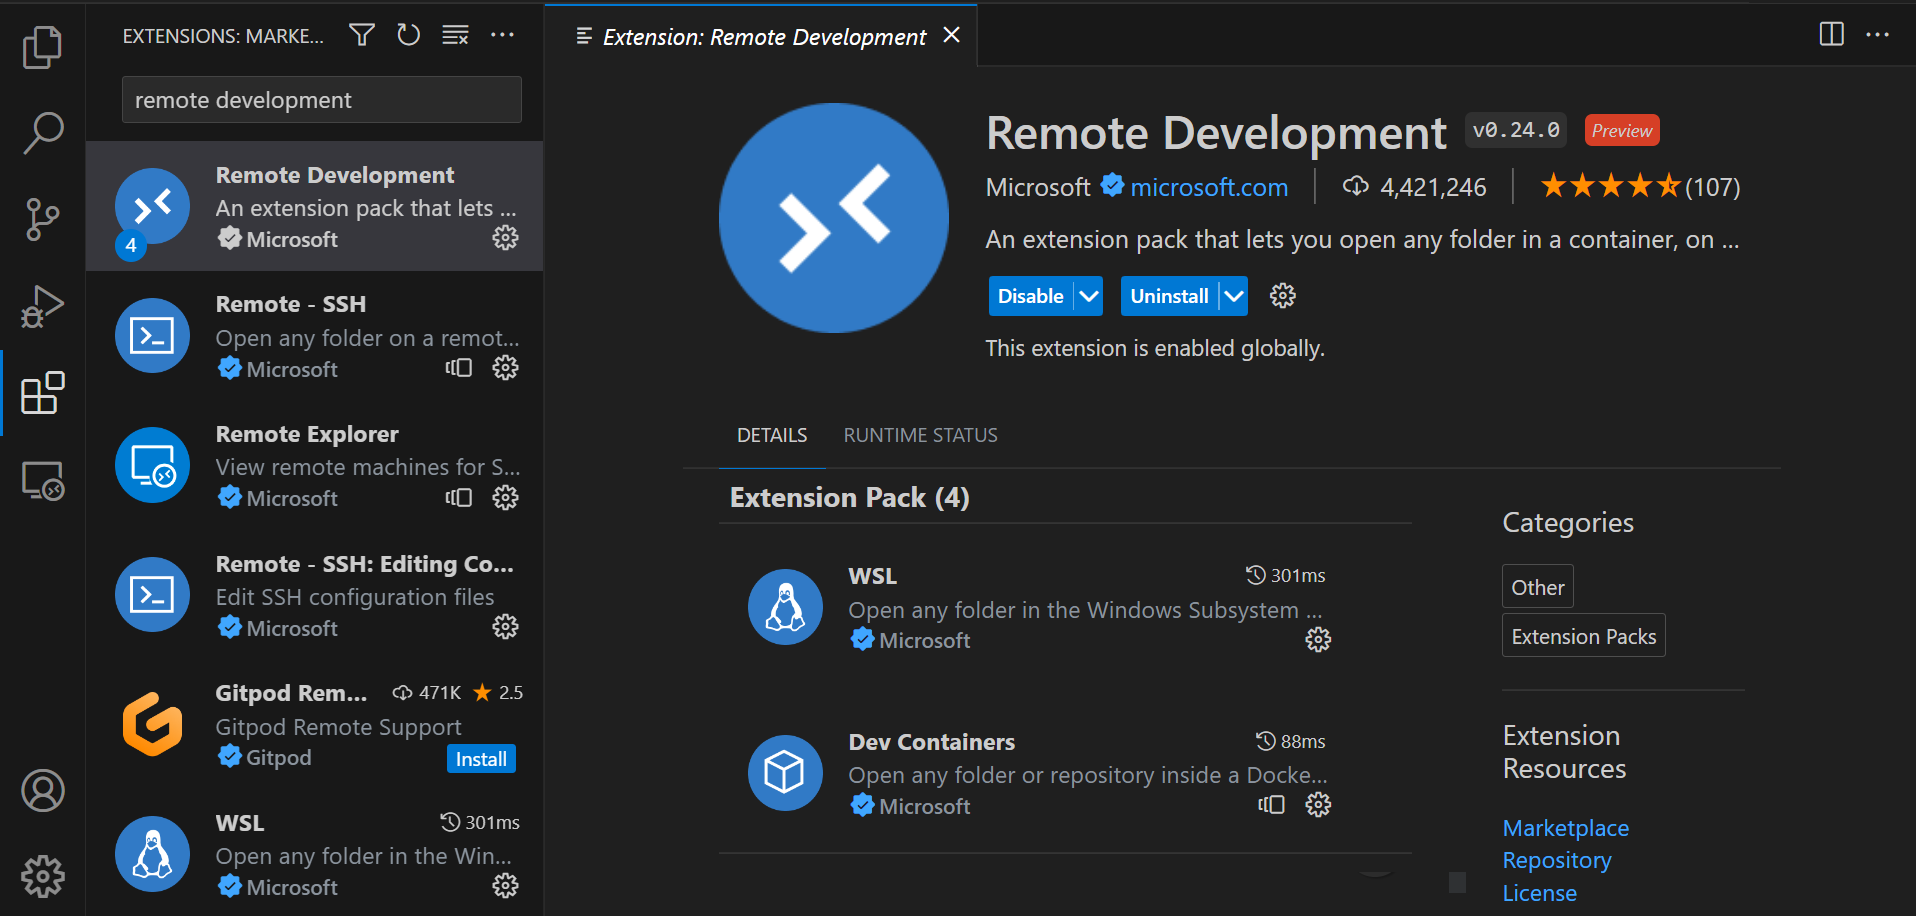
\includegraphics[width=0.8\linewidth]{extension.png}
        \caption{Remote Development Extension in VSCode}
        \label{fig:install_docker}
    \end{figure*}

    \item This alternative of the docker start command will start the container in the background without an interactive terminal:\\
    \codeIn{docker start svfproject}

    \item Attach to the docker container. 
    
    \begin{figure*}[htpb]
        \centering
        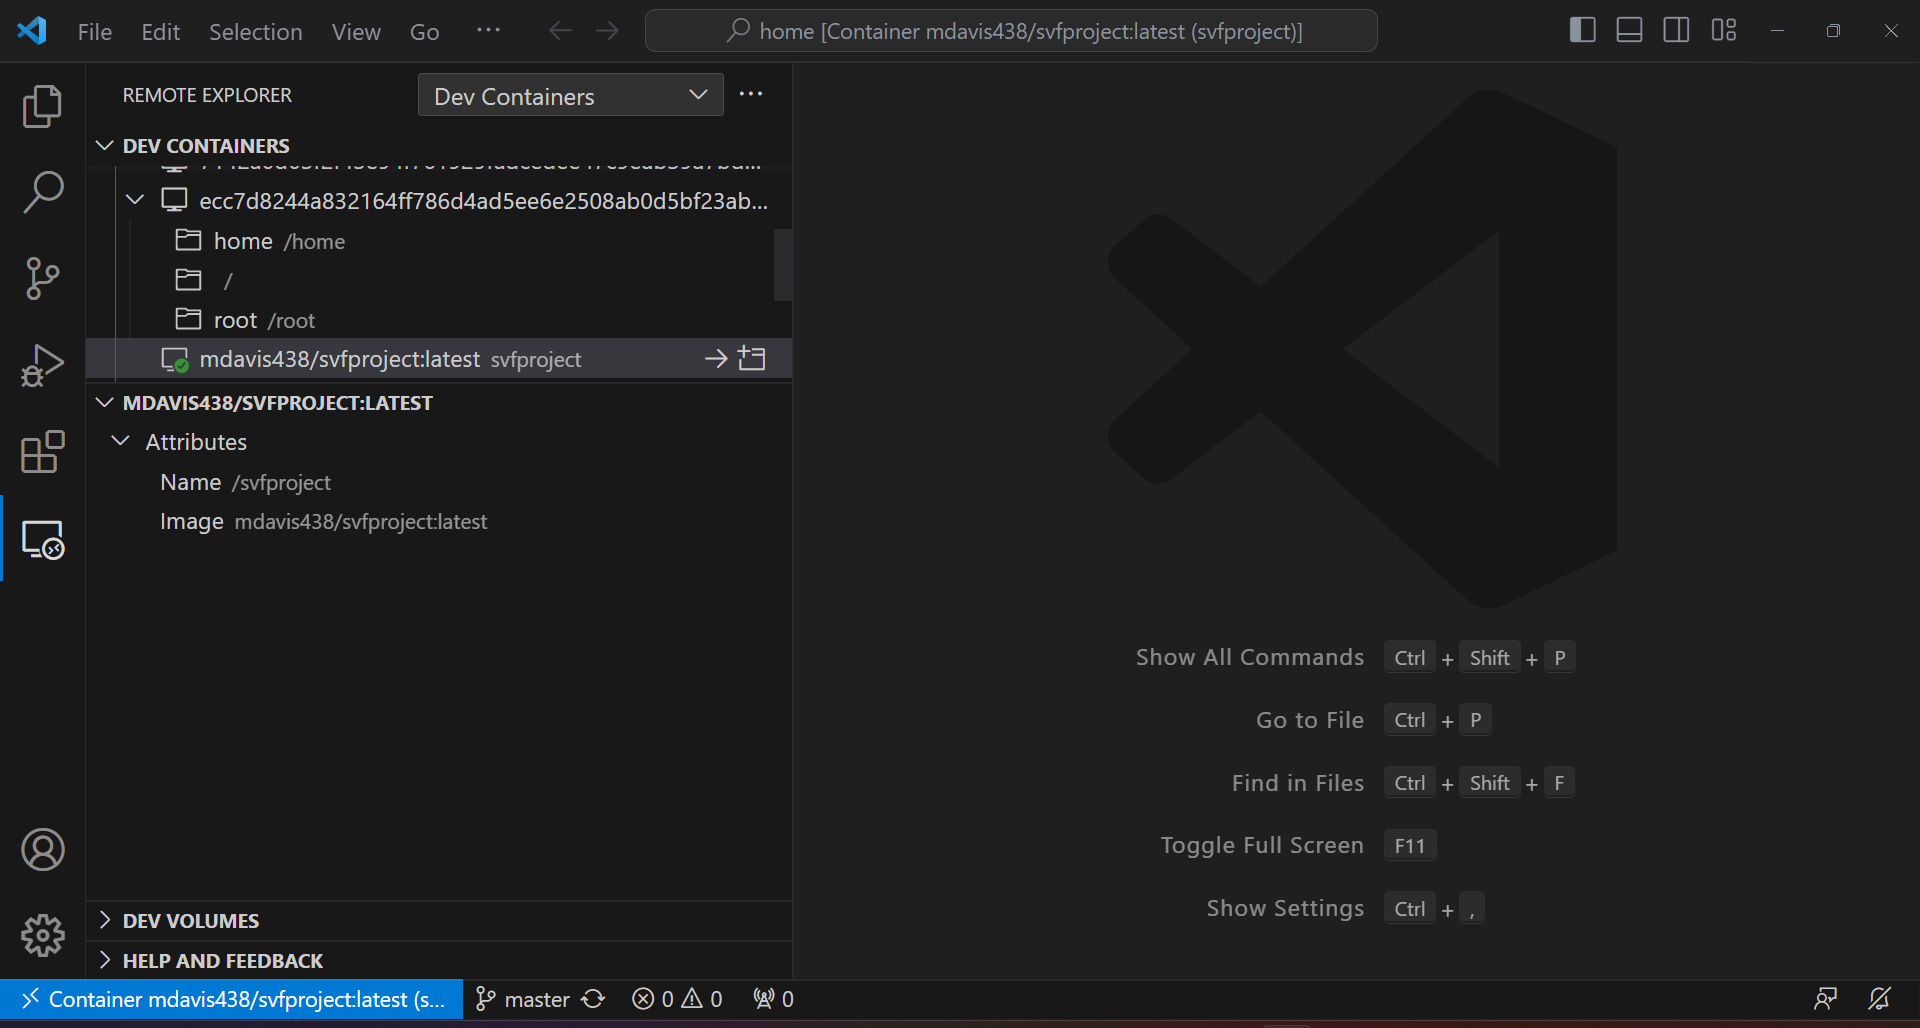
\includegraphics[width=0.8\linewidth]{attach.png}
        \caption{Dev Containers in VSCode}
        \label{fig:install_docker}
    \end{figure*}
    Open the Remote Explorer view from the left panel. Select "Dev Containers" in the dropdown at the top of the sidebar. This should list all of the docker containers available and currently running. Choose your project container ('svfproject'). VSCode will take some time to setup the connection and then open the container environment.

    More info on dev containers can be found \href{https://code.visualstudio.com/docs/devcontainers/containers}{here}. If you're curious you can follow this \href{https://code.visualstudio.com/docs/devcontainers/tutorial}{tutorial} but replace the example container instructions with our docker container.
    
\end{enumerate}

\subsubsection{Project Setup}
\begin{enumerate}
    \item To complete this project, you only need to modify the following file inside the container.\\\\
    \codeIn{$\sim$/project/src/project.cpp}\\
    
    \item After completing the code in this file you can build the project by first going to the directory ``\codeIn{$\sim$/project/}'' and then running the following commands\\\\
    \codeIn{source ./env.sh}\\
    \codeIn{./build.sh}\\

    \item This will generate the executable \codeIn{$\sim$/project/bin/svf-project}. The project can be run using the command\\\\    
    \codeIn{./test.sh [path/to/test.bc]}\\\\
    and will generate the \codeIn{out.txt} output file
    

\end{enumerate}
\section{Provided Code}

The only provided code is in the Docker container on Docker Hub, so there is no project directory provided. In the Docker container we have only provided the framework to build the project based on
the dependence of SVF libraries. There will only be a
placeholder \implementationFile file. In this file, you need to use the SVF framework to generate the ICFG graphs of
the input LLVM IR file. And you need to use SVF to identify the nodes
representing the \src () function call and \sink () function call.
Then your project should perform the reachability analysis and print the result to \codeIn{stdout}.

\section{Grading}
There are in total 100 points for this project.

\subsection{Correct Implementations (60 Points)}

Several test cases are given to you to test the correctness of your project under the \codeIn{$\sim$/project/test\_cases} directory.

You can run the script \codeIn{test.sh} to check the correctness of your
project for these test cases. For grading, there will be hidden test
cases for the project.

For each input test cases, your program is expected to print out the following outputs:
\begin{itemize}
    \item \textbf{First line:} The result whether the \src () function call can reach the \sink () function call (40 Points). If it is reachable, your program should print ``Reachable'', otherwise print  ``Unreachable''. Note that please print the EXACT text of ``Reachable'' or ``Unreachable''. For example, ``UnReachable'' is not an acceptable  output.  If your program provides correct answers to the reachability results, you can get 40 Points.
    \item \textbf{Following lines:} If there are $n$ traversal paths between the \src\  and \sink, your project should also print $n$ more lines. Each line 
    is a path from \src () to \sink () (20 Points). The path should have
    the following format, supposing that node 1 is the \src\  node and node 5 is the \sink\  node: \codeIn{$1-->2-->3-->4-->5$}. In the instance that the path or a portion is cyclic, annotate the cyclic region in the following format: \codeIn{$1-->Cycle[2-->3-->4]-->5$}. The exit node from the cycle must be correct, regardless if this duplicates nodes i.e. \codeIn{$1-->Cycle[2-->3-->4-->2]-->5$}. Correct program traversal paths will award 20 Points.
\end{itemize}

\subsection{Performance Evaluation (10 Points)}\label{sec:eval}
If your program can finish running each test case in 30 seconds, you will get 10 Points.

\subsection{Design (30 Points)}\label{sec:design}

In your final report, 
please briefly describe the following:
%
\begin{enumerate}
\item Details about how you generate the ICFG from the input LLVM IR.
\item Details about how you perform the reachability analysis.
\item Any known outstanding bugs or deficiencies that you were unable
  to   resolve before the project submission.
 \end{enumerate}

\section{Submission}\label{sec:sub}
To facilitate the grading, you should not modify
other files in the project directory!
On Canvas, submit a single ZIP file that contains:
\begin{itemize}
    \item The \implementationFile file
    \item The \codeIn{design.pdf} file described in Section~\ref{sec:design}.
    \item Any test cases you added. (This will not be graded.)
\end{itemize}
\textbf{We will only use the \implementationFile file to test the correctness of your implementation. If you modify other files, even if your code runs correctly on your local machine,
you will still get points deducted if it cannot run properly in our grading environment.}

\section{Collaboration}
%
We will award identical grades to each member of a given project team,
unless members of the team directly register a formal complaint.
%
We assume that the work submitted by each team is their work solely.
% 
Any questions about design and implementation should conducted solely with the instructors through office hours, email, etc.
%
Under no condition is it acceptable to use code written by another
team, or obtained from any other source.
%
As part of the standard grading process, each submitted solution will
automatically be checked for similarity with other submitted solutions and with other known
implementations.

\end{document}
